% !TEX encoding = UTF-8 Unicode 
% !TEX root = praca.tex

\chapter{Makieta sprzętowa}

Znaczącą częścią pracy jest makieta sprzętowa, została zaprojektowana i wykonana jako układ płytek drukowanych połączonych
przewodami stosowanymi powszechnie w elektronice w łączeniu układów na płytkach stykowych lub płytek deweloperskich
będących częścią prototypów urządzeń elektronicznych.


W skład makiety sprzętowej wchodzą:

\begin{itemize}

    \item \textit{KA-NUCLEO-F411CE} - płytka rozwojowa z mikrokontrolerem \textit{STM32F411CE} oraz układem programatora \textit{ST-Link/v2.1} \cite{NUCLEO} (rys. \ref{fig:f411_main} i \ref{fig:f411_stlink}),

    \item \textit{SparkFun Single Lead Heart Rate Monitor - AD8232} - płytka ze złączem na elektrody pomiarowe, układem \textit{AD8232} oraz filtrami analogowymi \cite{AD8232BS},

    \item \textit{Elektrody pomiarowe},

\end{itemize}


Makieta sprzętowa wykonana w pracy ma charakter prototypu urządzenia elektronicznego, jej elementy połączone są przewodami które można rozłączać i łączyć w dowolny sposób tak aby zmienić konfigurację urządzenia.

\begin{figure}[h!]
    \centering 
    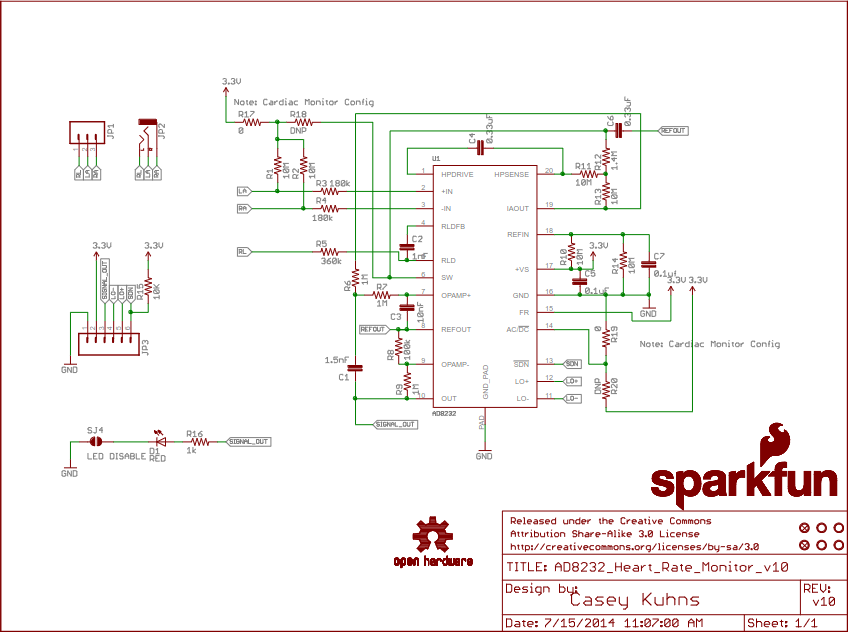
\includegraphics[scale=0.6]{pl/media/ad8232_sch.png}
    \caption{Schemat elektryczny płytki \cite{AD8232BS} zawierającej układ \textit{AD8232}}
    \label{fig:ad8232_sch}
\end{figure}

Do próbkowania i kwantyzacji sygnału z wyprowadzenia oznaczonego \textit{REFOUT} (rys. \ref{fig:ad8232_sch})
zastosowano kanał nr. 1 przetwornika \textit{ADC} tj. wyprowadzenie z oznaczeniem \textit{PA1} mikrokontrolera 
(rys. \ref{fig:f411_main}). Napięcie było mierzone wzlgędem masy (\textit{GND} na schematach).

W makiecie użyto również zestawu trzech diód (w jednej obudowie) o kolorach czerwonym, zielonym i niebieskim (\textit{RGB}, \textit{D2} - rys. \ref{fig:f411_main}) umożliwiających wyświetlanie dowolnej barwy złożonej z wymienionych składowych. Kolorowe diody użyte zostały do bardzo podstawowej komunikacji z użytkownikiem, informując np. o tym czy elektrody są prawidłwo podpięte.

Wyprowadzenia oznaczone \textit{SDN}, \textit{LO+} i \textit{LO-} (rys. \ref{fig:ad8232_sch}) zostały połączone odpowiednio 
do wyprowadzeń \textit{PB1}, \textit{PB6} i \textit{PB5} mikrokontrolera (rys. \ref{fig:f411_main}).

\begin{figure}[h!]
    \centering 
    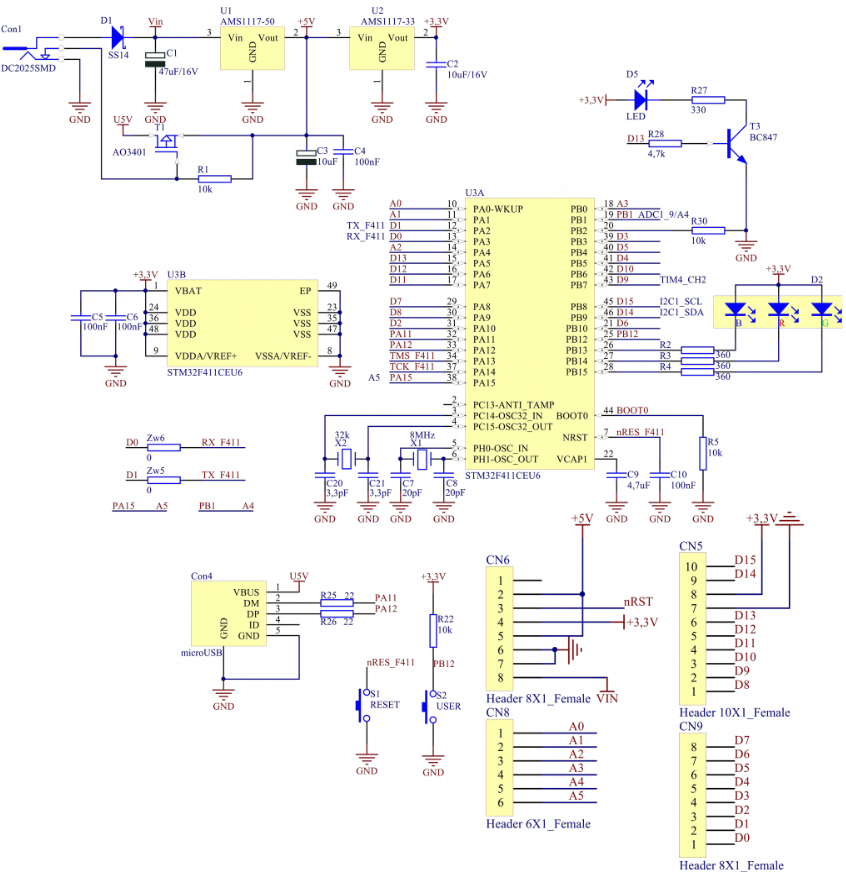
\includegraphics[scale=0.65]{pl/media/f411_main.png}
    \caption{Schemat elektryczny głównej części płytki \cite{NUCLEO} zawierającej mikrokontroler \textit{STM32F411CE}}
    \label{fig:f411_main}
\end{figure}

\begin{figure}[h!]
    \centering 
    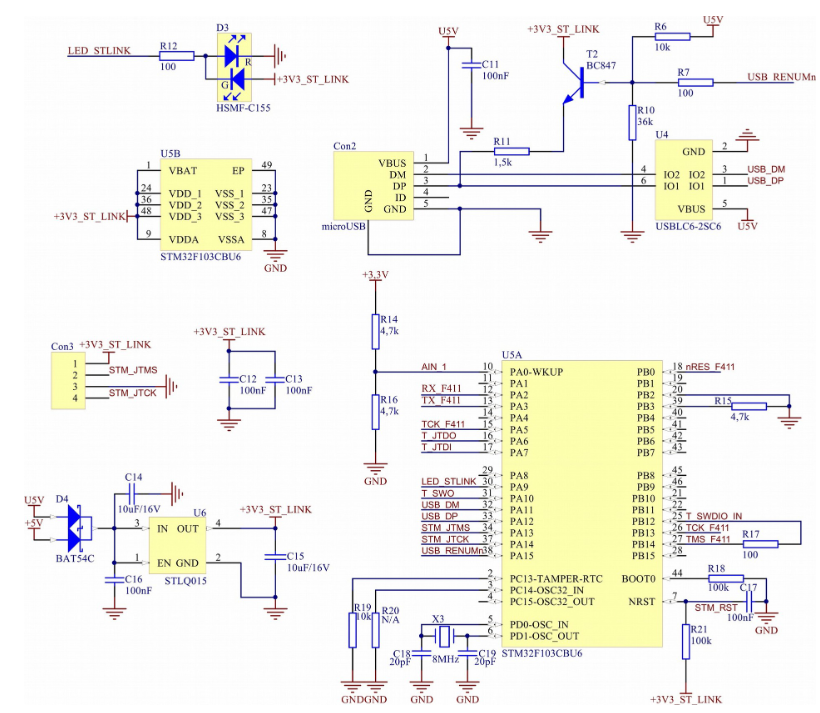
\includegraphics[scale=0.65]{pl/media/f411_stlink.png}
    \caption{Schemat elektryczny części płytki \cite{NUCLEO} zawierającej programator \textit{STLink/v2.1} 
    wraz z urządzeniem \textit{USB CDC}}
    \label{fig:f411_stlink}
\end{figure}

